% !Mode:: "TeX:UTF-8"

\chapter{魔方还原算法的研发与优化}

本章详细阐述了本课题在软件层面的工作与成果,主要体现在魔方还原算法的并行还原优化方面,本章是系统算法的核心所在。本章模块的主要工作包括两阶段算法的应用,并行还原优化等。

\section{开发环境简介}

本系统的开发在软件层次分为上位机和下位机两部分。其上位机程序部分是在Ubuntu 20.04.3 LTS的操作系统上使用Python语言并在JetBrains公司的Pycharm集成开发环境下进行魔方还原算法的开发;下位机程序部分首先在Windows10的操作系统上使用基于类C + + 语言在Arduino开发环境下进行指令接收、电机旋转等相关功能的开发,待开发结束后将代码烧录至Arduino Nano开发板上。

\subsection{Ubuntu 20.04操作系统}

Ubuntu 20.04.3 LTS (Focal Fossa)。Ubuntu 20.04是 Ubuntu 的第 8 个 LTS 版本,代号为"Focal Fossa",此次版本将会获得 5 年的技术支持,直至2025年4月,本次长期支持版本包含了诸多增强的安全特性,包括可防止低层攻击和包括可防止 rootkit 和低级攻击的安全启动。Ubuntu 20.04 LTS Beta 已将大部分核心软件包和工具链升级至新版本,包括正在使用的 Linux 5.4 内核,GNOME 3.36 桌面环境,文件系统升级至 ZFS 0.8.3。

以下是Ubuntu20.04的特点:GNOME 3.36 是默认的桌面系统;性能大幅度提高;拥有华丽的 Yaru 主题,同时也具有黑暗模式;改进的 ZFS 支持可以获得最新的 Linux 内核 5.4(LTS);增加了对 exFAT 的支持;改进硬件和图形支持;更新软件 Python 3.8.2;Wireguard 已被移植到 Linux 内核5.4,可以在 Ubuntu 20.04 上使用等。

\subsection{PyCharm集成开发环境}

PyCharm是一种Python语言的集成开发环境。该集成开发环境在先进代码分析程序的支持下,使其成为 Python 专业开发人员和刚起步人员使用的有力工具。PyCharm是用于Python脚本语言的最流行的IDE。除此之外,该集成开发环境提供了以下高级功能:代码补全、项目代码导航、代码分析、Git可视化、代码覆盖率、包装管理、本地历史、重构等。总的来说,PyCharm还是一款比较强大的IDE。

\subsection{PyQt5库}

Qt框架用C/C++语言编写的,PyQt是Qt框架的Python语言实现,是最强大的GUI库之一。在本系统中该库主要用于制作UI界面。其特性有以下几点:能够跨平台运行;基于高性能的Qt的GUI控件集;对Qt库进行完全封装;使用信号槽机制进行通信;提供一整套种类齐全的窗口控件等~\cite{28}。

PyQt5中的类包含很多模块与功能,其中QtWidgets类包含了一系列创建桌面应用的UI元素;QtTest提供了测试PyQt5应用的工具;QtXml包含了处理xml的类,提供了SAX和DOM等API的工具; QtSql提供了处理数据库的工具;QtMultimedia包含了处理多媒体的内容和调用摄像头API的类;QtPositioning包含了定位的类,可以使用卫星、WiFi甚至文本。

上述功能模块中,本系统只选用QtWidgets类,目的是制作一个简易美观的UI界面。除此之外还有一些人机交互功能更是凸显了本系统的实用性,对于系统使用者来说大大提高了使用便捷性。

\subsection{串口通信模块}

串口是计算机上一种非常通用的设备通信协议。而串口通信是指外设与计算机之间通过数据信号线等方式,设置波特率、停止位、校验位、字节大小等相关参数后按位进行传输数据的一种通讯方式。

本系统的串口通信模块使用USB2.0接口连接上位机与下位机,负责两端的通信~\cite{29},传输电机旋转的操作指令。PySerial模块封装了Python语言对串行端口的访问。

\section{系统目录规划表}

本系统将所有文件与目录放置在rubik文件夹下,该文件夹包含src文件夹以及系统运行的必要配置文件,src文件夹包含魔方块识别图片的images文件夹与系统运行的Python文件,images文件夹里包含魔方块颜色识别前后的marked和unmarked文件夹,marked文件夹存放识别并标记后的图片,unmarked文件夹存放识别前的图片。系统目录规划的具体情况如下表~\ref{tab:3-1}~系统目录规划表所示:

\begin{table}[H]
	\caption{系统目录规划表}\label{tab:3-1}
	\vspace{0.5em}
	\begin{center}
		{\wuhao
			\begin{tabular}{ll}
				\toprule
				目录 & 名称及说明	\\
				\midrule
				/rubik & 总目录,此目录存放系统的所有文件,包括环境配置文件等 \\
				/rubik/src & 用于存放上位机所有运行文件,包括业务逻辑代码等\\
				/rubik/src/images & 存放魔方块颜色识别图片的目录\\
				/rubik/src/images/marked & 存放识别并标记后的图片\\
				/rubik/src/images/unmarked & 存放识别前保存的图片\\
				\bottomrule
		\end{tabular}}
	\end{center}
	\vspace{-1.5em}
\end{table}

\section{系统算法流程图}

本系统的整体运作流程如下:首先通过摄像头获取魔方六个面的图像,再根据魔方块颜色识别算法对每个魔方块进行颜色识别,如果识别完全正确得到魔方块颜色序列后并计算出可行的解法,那么可直接执行魔方复原的操作。如果识别不完全正确,则需要根据魔方块位置和魔方块颜色的信息手动矫正识别结果,待矫正完所有错误颜色结果并得到可行还原解法之后即可执行魔方复原操作。该算法的流程图如下图~\ref{fig:3-1}~所示:

\begin{figure}[H]
	\centering
	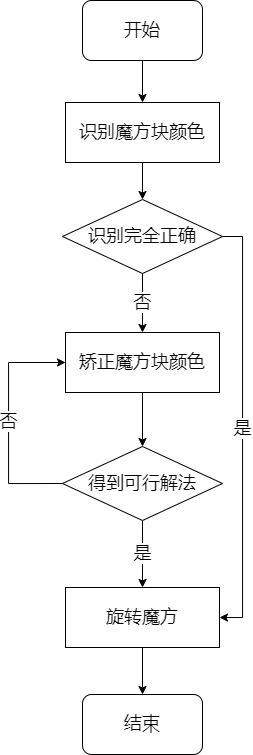
\includegraphics[width=0.2\textwidth]{3-1}
	\caption{系统流程图}\label{fig:3-1}
\end{figure}

\section{系统实现}

\subsection{可视化界面设计}

本论文中的界面设计部分首先通过QTCreator设计界面的大致结构,例如按钮、窗体等构件的分布,设计图如下图~\ref{fig:3-2}~所示,将设计图所生成的ui文件转换至py文件并微调参数后即是本系统的初始界面。

该设计图大致分为三个模块,界面最上方是图片显示模块,在系统运行后在该模块会显示摄像头捕捉到的四张图片;中间类似魔方展开图部分是魔方可视化模块,该模块将颜色识别后的结果与其背景颜色相结合,系统使用者可通过相应魔方块位置的背景颜色直观地了解魔方块颜色识别的结果,为后续魔方块颜色矫正过程提供了便捷。设计图界面最下方是操作模块,在该模块中提供识别、颜色矫正、还原可行性验证、魔方复原的功能,极大程度上减少魔方复原出错的可能性。

\begin{figure}[H]
	\centering
	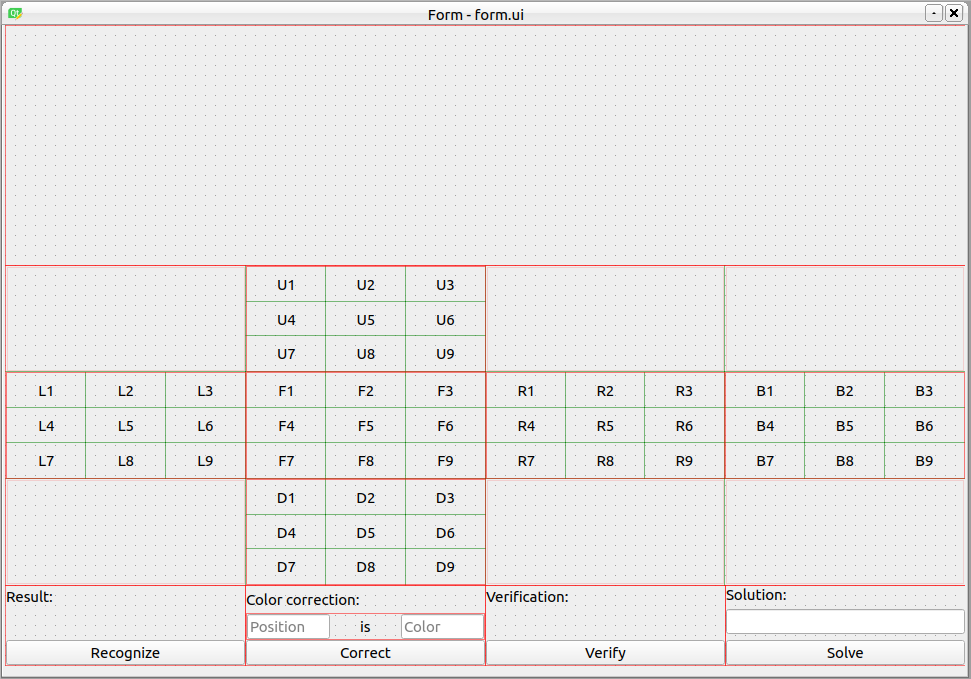
\includegraphics[width=0.9\textwidth]{3-2}
	\caption{可视化界面设计图}\label{fig:3-2}
\end{figure}

在可视化界面设计中,不同函数有不同的功能,其中包含初始化参数、设置构件布局及命名、配置构件颜色、设置按钮触发器等。详细的函数说明表如下表~\ref{tab:3-2}~所示:

\begin{table}[H]
	\caption{详细函数说明表}\label{tab:3-2}
	\vspace{0.5em}
	\begin{center}
		{\wuhao
			\begin{tabular}{cc}
				\toprule
				函数名称 & 主要功能	\\
				\midrule
				\_\_init\_\_ & 初始化参数 \\
				setupUi & 设置构件布局及命名\\
				setStyleSheet & 配置构件颜色\\
				retranslateUi & 设置构件显示的内容\\
				click\_connecting & 设置按钮触发器\\
				push\_recognize\_button & 魔方块颜色识别\\
				push\_correct\_button & 修正魔方块颜色结果\\
				push\_verify\_button & 验证还原可行性\\
				push\_solve\_button & 复原魔方\\
				solve\_rubik & 求解魔方复原步骤\\
				rec\_color & 魔方块颜色划分\\
				setLabel & 设置可视化界面中魔方块颜色\\
				mark\_img & 标记识别结果\\
				communicate & 串口通信\\
				push\_solve\_button & 复原魔方\\
				solve\_rubik & 求解魔方复原步骤\\
				\bottomrule
		\end{tabular}}
	\end{center}
	\vspace{-1.5em}
\end{table}

\section{魔方块颜色识别}

本系统的魔方块颜色识别模块基于OpenCV库,采用HSV颜色模型对魔方块进行颜色的判断。与RGB颜色模型相比,HSV颜色模型对亮度并不敏感,反而是RGB 颜色空间的三个分量都与亮度密切相关,即只要亮度改变,三个分量都会随之相应地改变,因此使用RGB颜色模型在某种程度上无法彻底摆脱环境亮度对颜色识别的影响。下图~\ref{fig:3-3}~表示的 HSV 颜色空间,圆柱体的横截面可以看作是一个极坐标系,其中色调用极坐标的极角表示,饱和度用极坐标的极轴长度表示,明度用圆柱中轴的高度表示。

\begin{figure}[H]
	\centering
	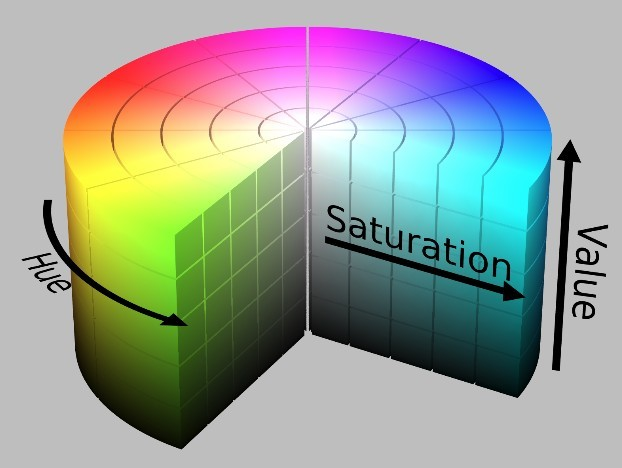
\includegraphics[width=0.6\textwidth]{3-3}
	\caption{HSV颜色空间示意图}\label{fig:3-3}
\end{figure}

HSV颜色空间比RGB颜色空间更容易跟踪某种颜色的物体,因此HSV颜色空间常用于分割指定颜色的物体。考虑到自然环境下获取的图像容易受自然光照、遮挡和阴影等情况的影响,因此采用HSV颜色模型对魔方块进行颜色识别。文献\mycite{30}\mycite{31}\mycite{32}是在HSV颜色空间下进行图像检索,例如电影中的镜头检测等,证明该颜色空间也可用于图像处理。文献\mycite{33}是基于HSV的机器人船舶导航系统,并且在低光照的情况下也可以很好的进行船舶导航。因此,周围环境光照的亮度强弱在HSV颜色空间下对系统的整体影响较小。

\begin{table}[H]
	\caption{HSV颜色分量范围表}\label{tab:3-3}
	\vspace{0.5em}
	\begin{center}
		{\wuhao
			\begin{tabular}{cccccccccccc}
				\toprule
				&黑&灰&白&\multicolumn{2}{c}{红}&橙&黄&绿&青&蓝&紫	\\
				\midrule
				$H_{min}$&0&0&0&0&156&11&26&35&78&100&125\\
				$H_{max}$&180&180&180&10&180&25&34&77&99&124&155\\
				$S_{min}$&0&0&0&\multicolumn{2}{c}{43}&43&43&43&43&43&43\\
				$S_{max}$&255&43&30&\multicolumn{2}{c}{255}&255&255&255&255&255&255\\
				$V_{min}$&0&46&221&\multicolumn{2}{c}{46}&46&46&46&46&46&46\\
				$V_{max}$&46&220&255&\multicolumn{2}{c}{255}&255&255&255&255&255&255\\
				\bottomrule
		\end{tabular}}
	\end{center}
	\vspace{-1.5em}
\end{table}

同时,考虑到本系统的摄像头角度及位置固定,因此在判断每个魔方块的颜色时并不需要做定位魔方块等工作,只需要人为标定每张图像中不同魔方块的固定范围即可。上表是HSV颜色分量范围表,对图像在HSV颜色空间的变量范围判断时,先是计算固定范围内像素点的分量平均值,接着判断其平均值在哪个范围内即可粗略判断颜色,最后根据不同的运行环境进行多次实验测试并修改具体分量边界值参数。该魔方块颜色识别的算法流程图如下图~\ref{fig:3-4}~所示:

\begin{figure}[H]
	\centering
	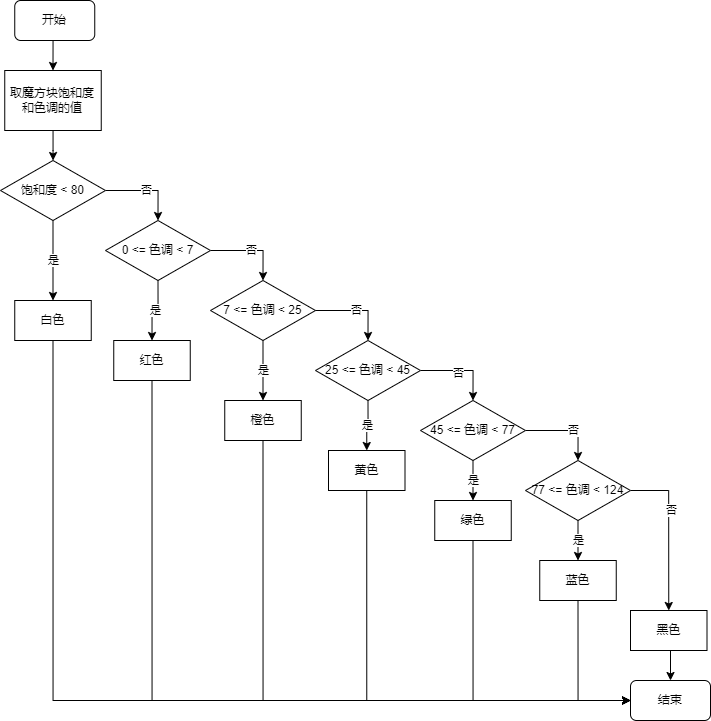
\includegraphics[width=\textwidth]{3-4}
	\caption{魔方块颜色识别流程图}\label{fig:3-4}
\end{figure}

在魔方块颜色识别中,包括捕捉魔方面图像、计算HSV平均值及颜色模型转换等函数,详细函数说明如下表~\ref{tab:3-4}~所示:

\begin{table}[H]
	\caption{函数清单}\label{tab:3-4}
	\vspace{0.5em}
	\begin{center}
		{\wuhao
			\begin{tabular}{cc}
				\toprule
				函数名称 & 主要功能	\\
				\midrule
				catch\_frames & 捕捉魔方面图像 \\
				cal\_hsv & 计算HSV各项平均值 \\
				detect & 颜色模型转换\\
				print\_hsv & 输出HSV颜色模型结果\\
				\bottomrule
		\end{tabular}}
	\end{center}
	\vspace{-1.5em}
\end{table}

下列四组图展示的是不同视角的摄像头处理前后的图片。每组右侧图片中的绿色矩形代表的是每个魔方块的像素范围,下列四组图片中,一共有48个绿色矩形,对应六个面的八个魔方块。

\begin{figure}[H]
	\centering
	\subfigure{
		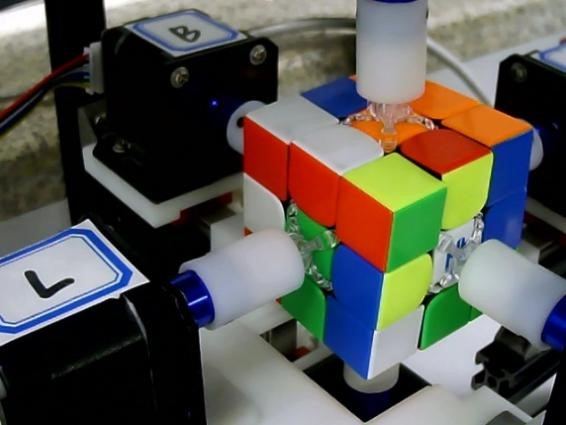
\includegraphics[width=0.4\textwidth]{3-5}}
	\subfigure{
		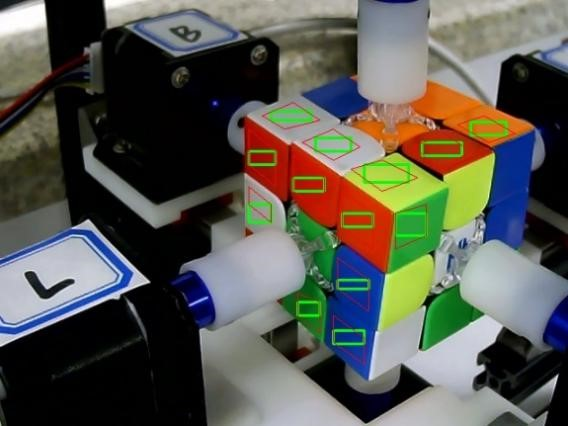
\includegraphics[width=0.4\textwidth]{3-5.1}}
	\caption{左上方视角原图(左)与处理后图片(右)}\label{fig:3-5}
\end{figure}

\begin{figure}[H]
	\centering
	\subfigure{
		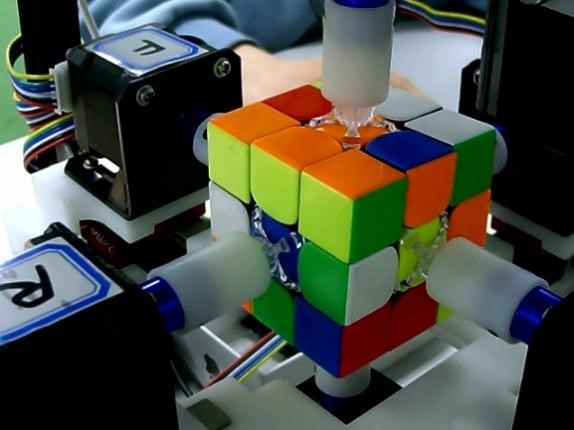
\includegraphics[width=0.4\textwidth]{3-6}}
	\subfigure{
		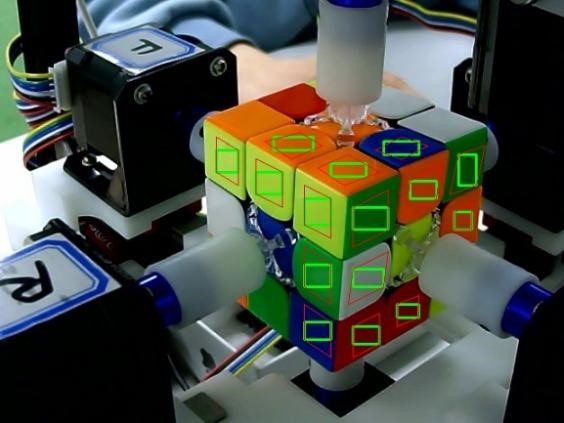
\includegraphics[width=0.4\textwidth]{3-6.1}}
	\caption{右后方视角原图(左)与处理后图片(右)}\label{fig:3-6}
\end{figure}

\begin{figure}[H]
	\centering
	\subfigure{
		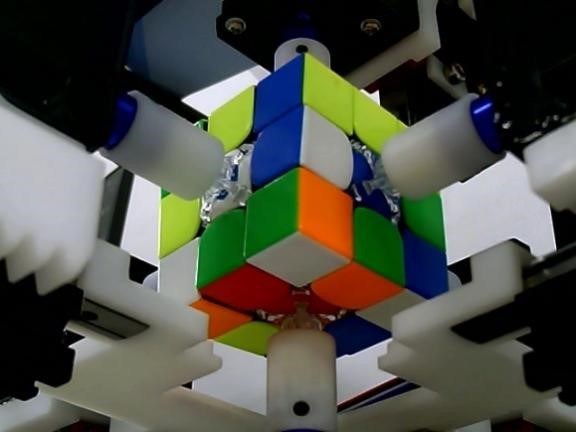
\includegraphics[width=0.4\textwidth]{3-7}}
	\subfigure{
		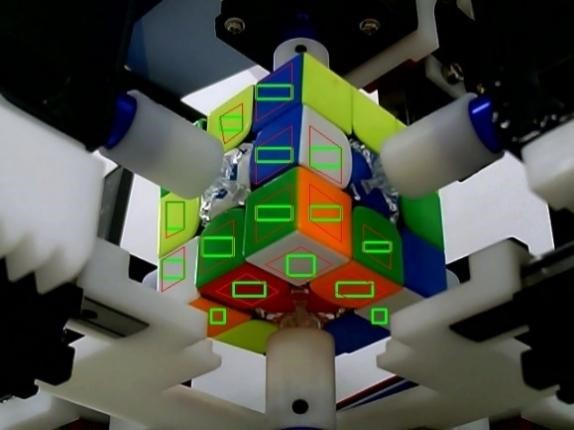
\includegraphics[width=0.4\textwidth]{3-7.1}}
	\caption{右下方视角原图(左)与处理后图片(右)}\label{fig:3-7}
\end{figure}

\begin{figure}[H]
	\centering
	\subfigure{
		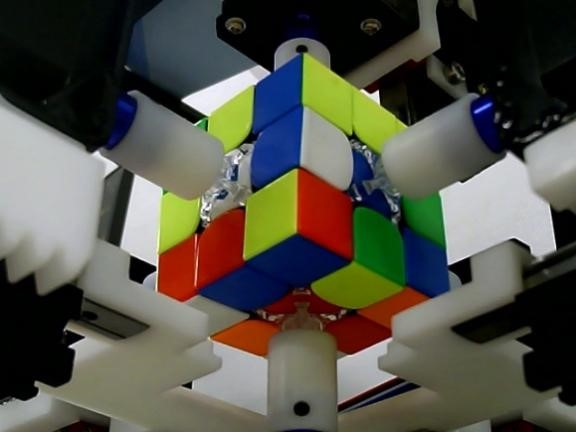
\includegraphics[width=0.4\textwidth]{3-8}}
	\subfigure{
		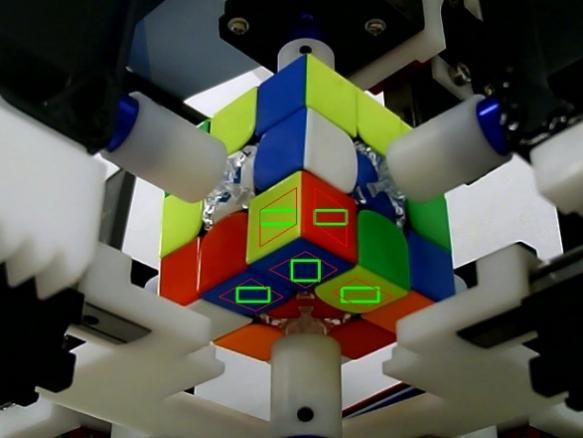
\includegraphics[width=0.4\textwidth]{3-8.1}}
	\caption{右下方视角原图(左)与处理后图片(右)}\label{fig:3-8}
\end{figure}

\subsection{Kociemba算法}

Kociemba算法,即两阶段算法,是由Thistlethwaite算法演变而来的。该算法采用降解子群~\cite{34}的核心思想将魔方复原分为四个步骤:

\begin{gather}
	G0 =<U,D,L,R,F,B>,\\
	G1 =<U,D,L,R,F2,B2>,\label{equ:3-2}\\
	G2 =<U,D,L2,R2,F2,B2>,\\
	G3 =<U2,D2,L2,R2,F2,B2>,\\
	G4 =<I>\text{(还原态)}.
\end{gather}

其中 U,D,L,R,F,B 分别代表顶面、底面、左面、右面、前面或后面旋转90°,如果字母后面紧跟数字 2 ,则代表旋转180°,例如 U2 意为顶面旋转180°。

以公式~\ref{equ:3-2}~为例,G1 子群代表的是由魔方顶面、底面、左面或右面旋转 90° 与前面或后面旋转 180° 任意组合后可还原魔方的魔方状态。换言之,当 G1 子群状态的魔方复原过程中,不允许出现魔方前面、后面旋转 90° 的情况。

上述各个子群降解过程中,其子群状态数变化如下表所示,影响因子意为降解至当前子群状态数缩小的倍数。

\begin{table}[H]
	\caption{子群状态数变化表}\label{tab:3-5}
	\vspace{0.5em}
	\begin{center}
		{\wuhao
			\begin{tabular}{ccc}
				\toprule
				群 & 状态数 & 影响因子	\\
				\midrule
				$G0=<U,D,L,R,F,B>$ & $4.33 \times 10^{19}$ & / \\
				$G1 =<U,D,L,R,F2,B2>$& $2.11 ×10^{16}$ &$2048(2^{11})$\\
				$G2 =<U,D,L2,R2,F2,B2>$&$1.95 ×10^{10}$&$1082565\left(\frac{12!}{8!\times4!\times3^7}\right)$\\
				$G3 =<U2,D2,L2,R2,F2,B2>$&$6.63 ×10^5$&$29400\left(\frac{8!}{4!\times4!}\times2\times3\right)$\\
				$G4 =<I>\text{(还原态)}$&$1$&$663552\left(\frac{4!^5}{12}\right)$\\
				\bottomrule
		\end{tabular}}
	\end{center}
	\vspace{-1.5em}
\end{table}

而Kociemba算法是分别将上述Thistlethwaite算法的前两个阶段合并为一个阶段,后两个阶段合并为另外一个阶段,在前后两个阶段合并的过程中都使用了在A*算法基础上加入迭代加深思想的IDA* 搜索算法~\cite{35}~\cite{36}。迭代加深~\cite{37}的操作可以保证搜索树上面的任何一个节点都可以获得精确的启发函数值。

本课题研究的算法内容是搭建借助两阶段算法应用至本魔方复原系统并采用部分并行的方式优化其还原步骤。

第一阶段:如果在拧魔方的时候不使用$\{R,R',L,L',F,F',B,B'\}$,那么会生成一个状态子集。这个子集我们用$G1=<U,D,R2,L2,F2,B2>$表示。在这个子集里面,角块和边块的方向是不会改变的,并且这点可以在盲拧中体会到。那就是说,对于一个块(边块或角块)而言,其方向是不会改变的。而魔方顶面与底面之间夹心的那四块边块仍然会保留在魔方顶面与底面之间。自然,魔方顶面与底面的边角块仍然会处在魔方顶面与底面。在第一阶段的搜索中,本算法会查找能把一个打乱的魔方变成G1状态的步法。那就是说,做完该步后,整个魔方边/角块方向都被纠正。在这个抽象的空间里,移动魔方一步会把代表魔方状态的三维组$(x,y,z)$变成$(x',y',z')$,所有G1状态的魔方都拥有相同的三位组$(x0,y0,z0)$,而这就是第一阶段搜索的目标。在 Cube Explorer 2中,它会给出需求解的魔方确切的达到G1状态的最少步数。这种启发式的算法可以在产生解法的时候提前剪枝,不需要等待一段非常非常长的时间来等结果。这种启发式的算法 h1使用的是基于内存的查表方法~\cite{38},最多允许提前12步做出判断剪枝。

第二阶段:在该阶段搜索中,会使用G1步法$\{U,D,R2,L2,F2,B2\}$来复原魔方。实际上就是复原八个角块,魔方顶面与底面的八个边块和魔方顶面与底面夹心的那四块的位置。启发式函数 h2(a,b,c) 只对复原六面的步法长度内的情况做出评估,因为G1子集里面的情况实在太多了。本算法不会在找到上面的解法后停止,而是会继续的在第一阶段的结果基础上继续展开第二阶段的搜索。举一个例子,如果上面的解法找到第1阶段需要10步,第2阶段需要12步,但后面搜索的结果可能是第1阶段11步,而第2阶段变成了5步。第1阶段的步法长度增加了,但第2阶段的步法减少了。如果第2阶段的步法长度减少到0。那么这个解法是优化完毕的,算法结束。 但是当前的两阶段搜索算法并不能在所有的情况下都找到最优解,在这种情况下我们必须倒回头,继续做一次二阶段搜索。这会增加相当多大的时间。

在该两阶段算法中,A*算法的启发函数进行初始化操作的同时会生成一个映射表,然后以魔方的原始状态为起点进行若干次操作,组成一颗操作树,显而易见,其根节点为魔方的原始状态。遍历操作树上面的所有节点,也就是每一个状态,从表上可以映射为一个启发函数值,其值的大小就为节点的深度。因为此时魔方的状态就是魔方在原始状态下通过其树的深度值次数的操作结果,经过相反的操作即可还原魔方。

同时,操作树上每个节点向上搜索必然存在状态相同的不同节点,因为启发函数的值应该为最小值才可以保证精度,因此,我们在遍历操作树的时候,使用广度优先搜索,保证浅层的节点先被记录,而深层同状态的节点因为已经存在映射关系而会被忽略。

得到映射表之后,在调用启发函数的时候,根据当前的魔方状态,经过查表可以获得启发函数的值,使用A*算法判断魔方的下一个判断即可,同时因为迭代加深的缘故,节点的判断函数都是准确的,而且不需要记录对未搜索的可达的节点。

本系统使用基于Python语言编程的Kociemba算法,以顶面、右面、前面、底面、左面与背面的顺序依次输入其颜色所代表的方位,即可得到魔方复原的步骤。

\subsection{并行旋转优化算法}

由魔方还原算法得出魔方求解步骤后,上位机将还原指令通过USB串口发送至下位机,下位机接收到其指令后,对该指令进行并行优化处理,根据不同情况执行不同旋转步骤。该算法的算法流程图如下图~\ref{fig:3-9}~所示:

\begin{figure}[H]
	\centering
	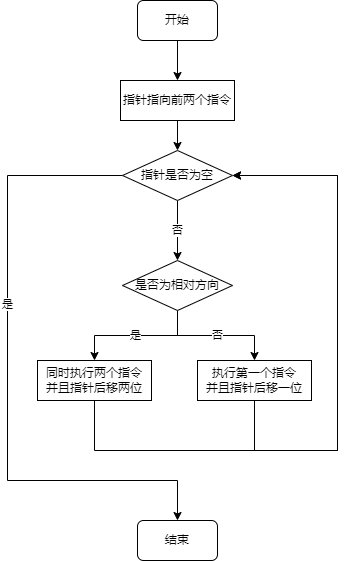
\includegraphics[width=0.4\textwidth]{3-9}
	\caption{并行优化算法流程图}\label{fig:3-9}
\end{figure}

\noindent 该算法流程如下所示:

\begin{enumerate}[itemsep=2pt,topsep=0pt,parsep=0pt]
	\item 新建两个指针指向还原指令中的前两个指令。
	\item 判断指针是否为空。若为空,结束该算法;若不为空,跳转至步骤3。
	\item 判断指针指向的两个指令是否控制相对方向的旋转,即U与D、L与R、F与B。如果是,跳转至步骤4,如果不是,跳转至步骤5。
	\item 同时执行两个指令并使指针后移两位。跳转至步骤2。
	\item 执行第一个指针指向的指令并使指针后移一位。跳转至步骤2。
\end{enumerate}

\section{系统界面截图}

\subsection{初始界面}

本系统的整体界面是由图~\ref{fig:3-2}~的整体设计图转化而来的。

本系统的界面一共包含三个部分:界面最上端是图片显示部分,位于界面中心位置是魔方颜色模拟部分,下端是系统操作部分。

系统开始运行后,其初始界面如下图~\ref{fig:3-10}~所示。点击Recognize按钮,本系统便开始进行魔方块颜色识别环节。在该环节,三个摄像头分别从左前、右前、右后方三个角度获取四张照片从而对各个魔方块进行颜色识别。

\begin{figure}[H]
	\centering
	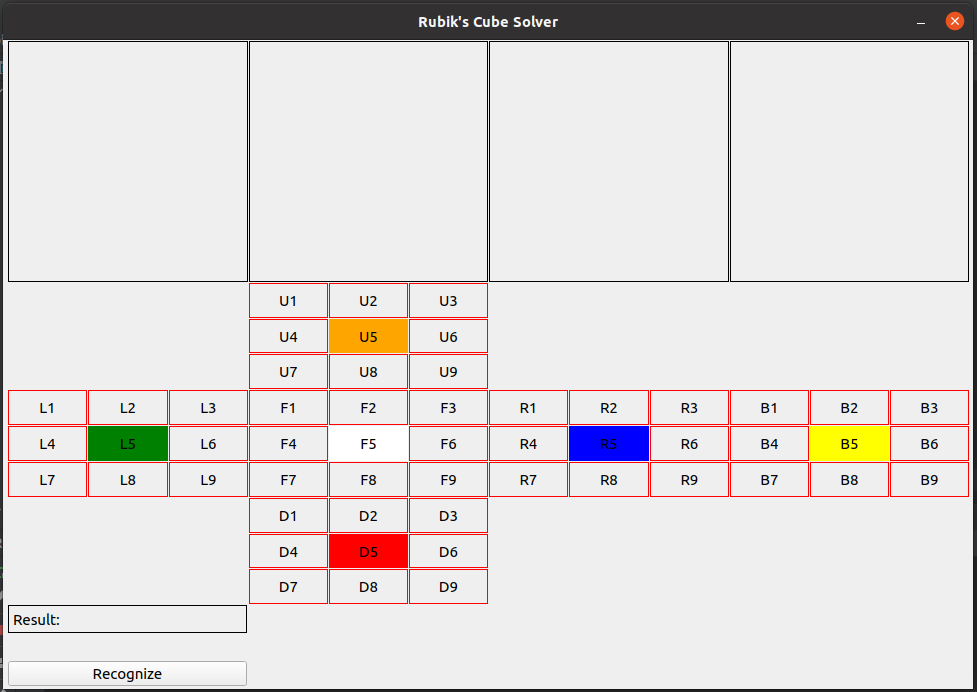
\includegraphics[width=0.95\textwidth]{3-10}
	\caption{系统初始界面}\label{fig:3-10}
\end{figure}

\subsection{颜色矫正}

对于颜色矫正部分,该界面如下图~\ref{fig:3-11}~所示。魔方块颜色识别完成后,系统界面上端会显示摄像头捕捉并标注候选框后的四张图像;系统界面中间部分会显示对应位置的颜色,例如L1位置的背景色是橙色,这代表着魔方左侧第一块的颜色为橙色;而当系统不能完全正确识别魔方块时,系统下端出现颜色修正以及可行性验证按钮。

本系统可对所有魔方块的颜色进行手工矫正,在颜色矫正栏输入魔方块位置与颜色即可对修改相应魔方块的识别颜色,例如在下图的文本框中输入R1与Red并点击Correct按钮,系统中间部分R1位置的魔方块背景色会被更改为红色,同时魔方块颜色序列中的相应位置也会被修改成红色,因此实现人工更正识别结果,可进一步增加系统的还原准确性。

\begin{figure}[H]
	\centering
	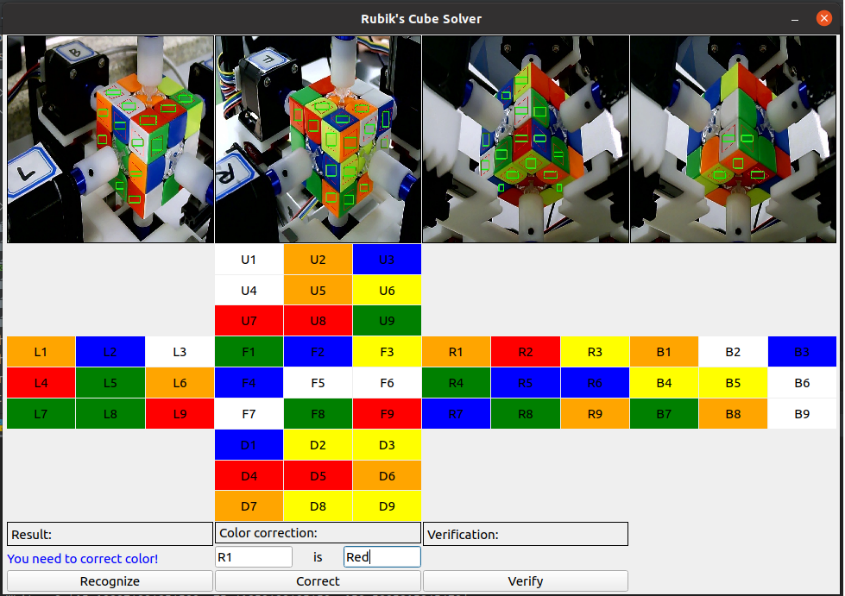
\includegraphics[width=0.95\textwidth]{3-11}
	\caption{颜色矫正界面}\label{fig:3-11}
\end{figure}

\subsection{还原可行性验证}

在上述的魔方块颜色矫正步骤之后,R1位置的魔方块背景色被更改为红色,如下图~\ref{fig:3-12}~所示。此时,系统可再次对校正后的魔方块颜色进行还原算法的求解。

如果矫正后仍然不能得到可行的还原步骤,那么证明并没有完全矫正正确,仍然需要重复颜色矫正操作。

如果系统提示Solved,则证明已经得到可行的复原步骤,下一步点击Solve按钮即可进行还原操作。

\begin{figure}[H]
	\centering
	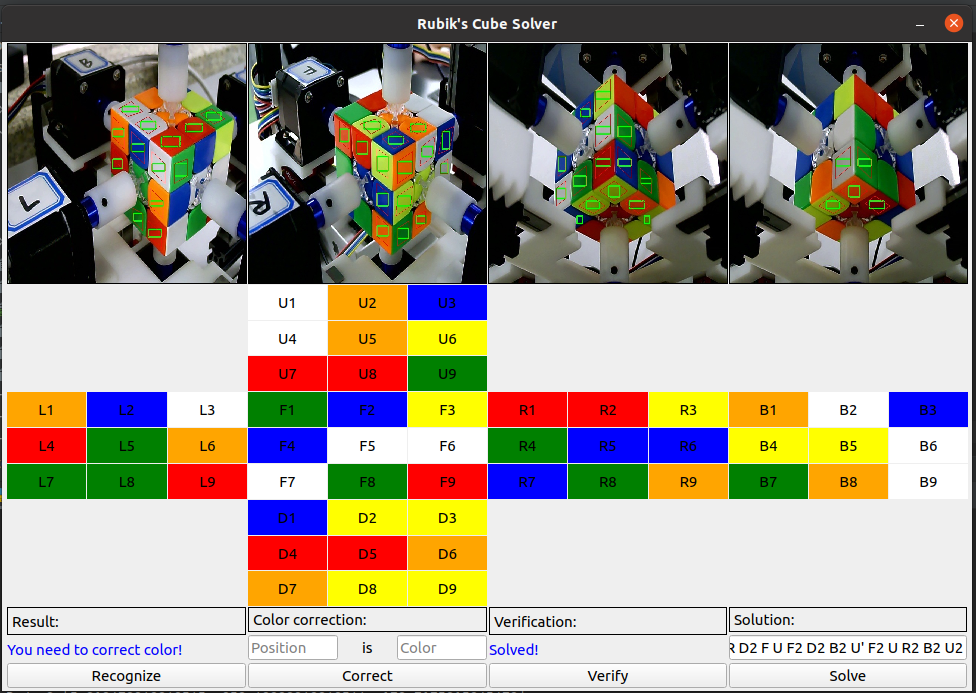
\includegraphics[width=0.95\textwidth]{3-12}
	\caption{还原可行性效果图}\label{fig:3-12}
\end{figure}

\subsection{魔方块还原}

在魔方块还原部分,不管是识别完全正确还是魔方块颜色矫正完成后得到可行的复原步骤,都需要执行魔方块还原操作。

在本系统得到魔方还原操作的序列后,点击Solve按钮后即可发送电机还原旋转指令对打乱的魔方进行还原,如下图~\ref{fig:3-13}~所示。

\begin{figure}[H]
	\centering
	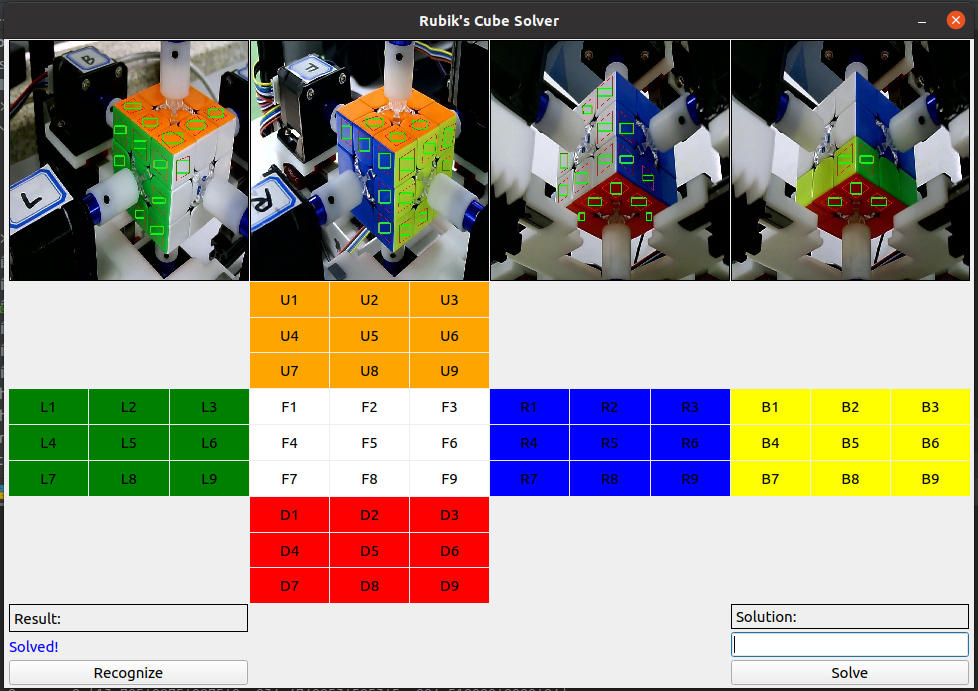
\includegraphics[width=0.95\textwidth]{3-13}
	\caption{魔方块还原结果界面}\label{fig:3-13}
\end{figure}

\section{本章小结}

本章首先简要介绍系统的开发平台和环境配置,接着列举系统目录规划表以及系统整体算法的流程图,再详细介绍本系统的界面设计,本系统使用的两阶段还原算法以及设计并行优化旋转操作策略。最后根据系统的不同功能截图展示本魔方复原系统的界面。